\documentclass[a4paper]{article}

\usepackage{amsmath,tikz}
\usepackage{babel}
\usepackage[utf8]{inputenc}
\usepackage[T1]{fontenc}
\usepackage{tikz}
\usepackage[top = 1cm, bottom = 1cm, left = 1cm, right = 1cm]{geometry}

\begin{document}

\begin{center}
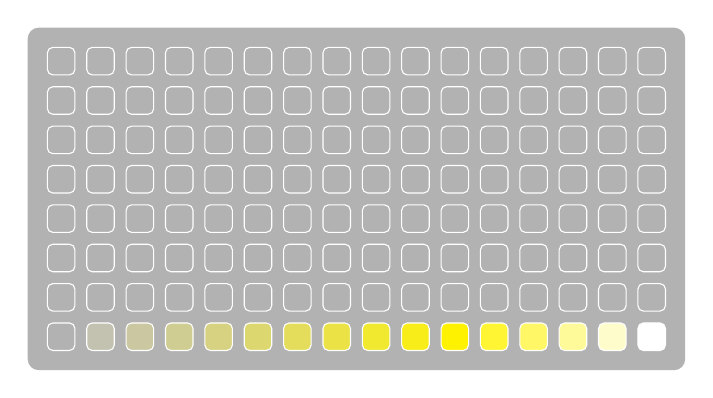
\begin{tikzpicture}[scale = 0.5]
  \fill[black!30!white, rounded corners] (0.3,0.3) rectangle (17,9);

  
  \colorlet{c0}{black!30!white}
  \colorlet{c1}{black!30!white!90!yellow}
  \colorlet{c2}{black!30!white!80!yellow}
  \colorlet{c3}{black!30!white!70!yellow}
  \colorlet{c4}{black!30!white!60!yellow}
  \colorlet{c5}{black!30!white!50!yellow}
  \colorlet{c6}{black!30!white!40!yellow}
  \colorlet{c7}{black!30!white!30!yellow}
  \colorlet{c8}{black!30!white!20!yellow}
  \colorlet{c9}{black!30!white!10!yellow}
  \colorlet{c10}{yellow}
  \colorlet{c11}{yellow!80!white}
  \colorlet{c12}{yellow!60!white}
  \colorlet{c13}{yellow!40!white}
  \colorlet{c14}{yellow!20!white}
  \colorlet{c15}{yellow!0!white}
    

  \foreach \x \y \z in {
    1/1/c0,
    2/1/c1,
    3/1/c2,
    4/1/c3,
    5/1/c4,
    6/1/c5,
    7/1/c6,
    8/1/c7,
    9/1/c8,
    10/1/c9,
    11/1/c10,
    12/1/c11,
    13/1/c12,
    14/1/c13,
    15/1/c14,
    16/1/c15}{
      \fill[fill = \z, rounded corners=2pt] (\x-0.2,\y - 0.2) rectangle (\x + .5, \y + .5) {};
    }
    

 % draw after filling
  \foreach \x in {1,...,16}
    \foreach \y in {1,...,8}
    {\draw[draw = white, rounded corners=2pt] (\x-0.2,\y - 0.2) rectangle (\x + .5, \y + .5) {};
    }
    
      
\end{tikzpicture}
\end{center}

\end{document}

%%% Local Variables:
%%% mode: latex
%%% TeX-master: t
%%% End:
